\begin{figure}
\centering
\fbox{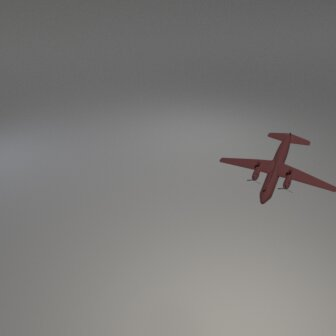
\includegraphics[width=0.4\linewidth]{figures/samples/single_object_6dof.jpg}}
\begin{minted}[breaklines]{python}
add(loc=(6.355, -4.600, 4.206), color='Mahogany', shape='jet', material='matte', rotation=(0.941, -0.337, 0.022, -0.303, -0.815, 0.493))
\end{minted}
\caption{\textbf{Single-Object 6-DoF Train Sample.} (\cref{sssec:single_6dof})}
\label{fig:code_single_6dof}
\end{figure}